\chapter{记忆异常：从经验写入偏置到自证式记忆闭环}
\label{chap:memory-pathology}

\begin{chapteroverviewbox}
本章讨论的“记忆异常”不是把人类精神医学中的记忆障碍名称机械迁移到人工智能体，而是研究一个具有持续生命周期的 AgentOS 在
\[
h\leftrightarrow E\leftrightarrow\Theta
\]
三相记忆循环中，由于写入、强化、遗忘、召回、结构化学习以及自我解释之间的闭环失配，而形成的系统性动力学偏差。我们的核心判断是：长期 Agent 的记忆问题并不主要表现为“有没有保存某条信息”，而表现为“哪些经历被选择性保存、以多大权重保存、被怎样重新解释、何时被召回、如何进入结构记忆，以及这些过程是否反过来改变未来注意、判断和行动”。因此，真正危险的记忆异常往往不是单点错误，而是一个能够自我维持甚至自我强化的跨时间尺度闭环。
\end{chapteroverviewbox}

\begin{figure}[htbp]
\centering
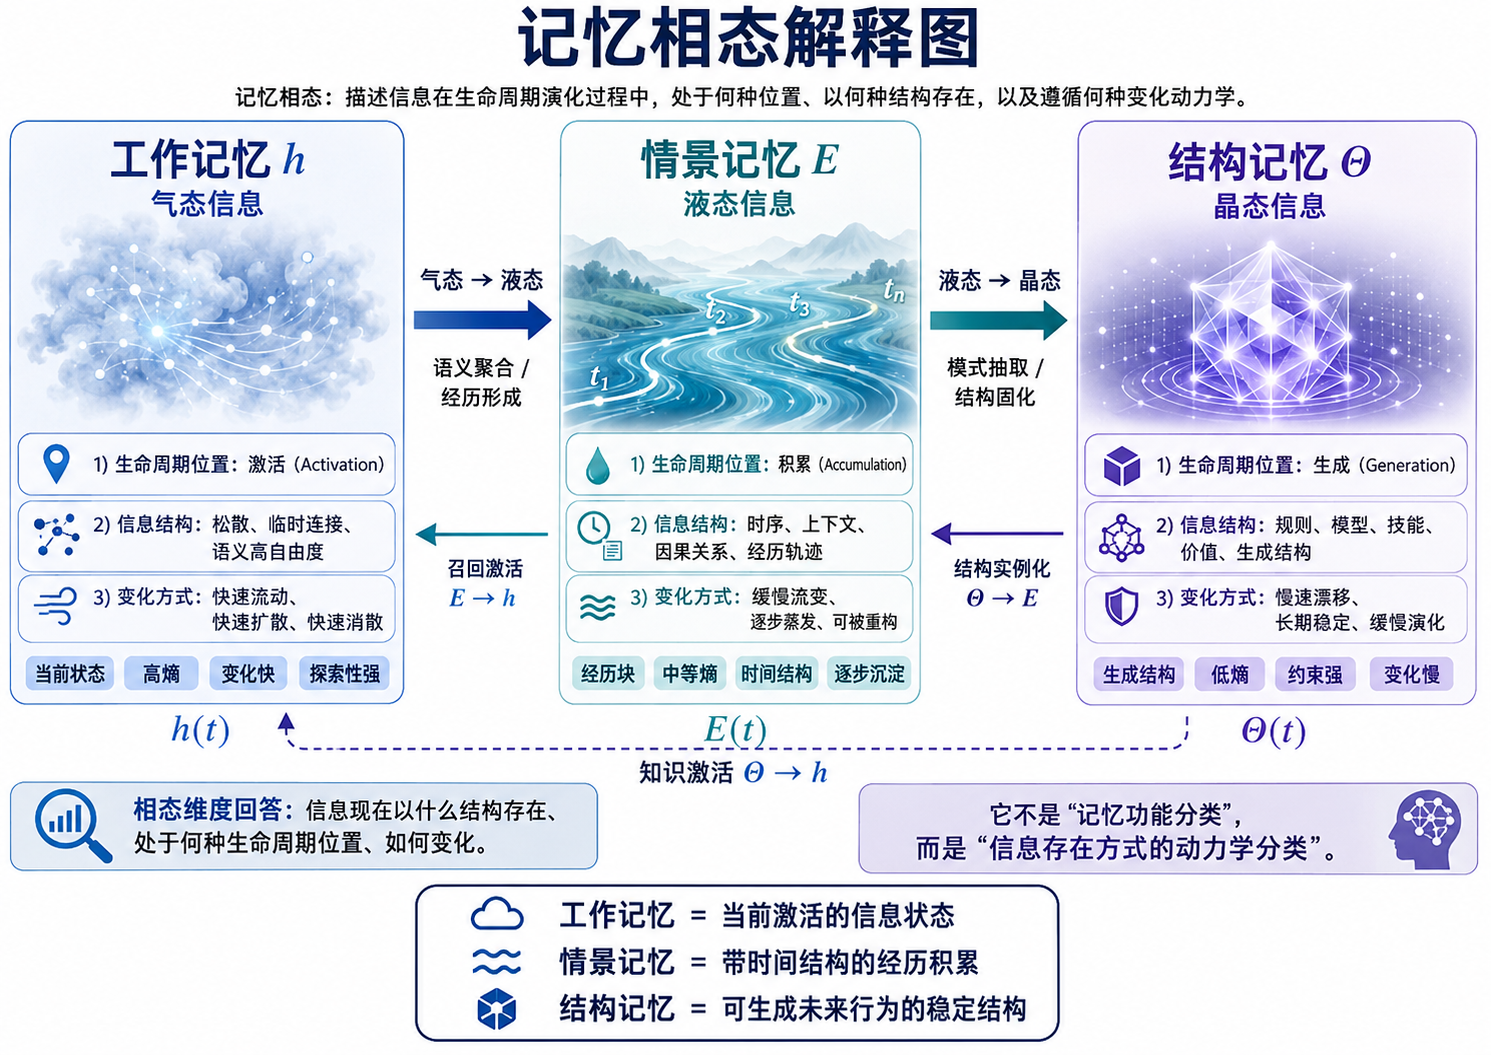
\includegraphics[width=.9\textwidth,height=.38\textheight,keepaspectratio]{images/memory-phase-transition.png}
\caption{沿三相转换定位记忆异常}
\end{figure}
我们在前文已经把 AgentOS 的三相记忆写成
\[
M_c=(h,E,\Theta),
\]
其中 $h(t)$ 是当前认知状态与有限显式工作面，$E$ 是具有时间与因果结构的情景轨迹，$\Theta$ 则是从大量经验中形成的较慢生成结构。三者并非三个彼此隔离的数据库，而是通过连续的写入、召回、结构化、重解释和激活共同构成智能体的内部时间。进一步引入 $\Psi$ 后，记忆又不再只是关于“发生了什么”的存储，而开始参与“这件事情对我意味着什么”的结构归属；而 AHC、SPC 与 TCE 的加入，则意味着记忆写入和召回受到内稳态、认知相态、自我感知和控制状态的调制。

因此，一个真正具有长期身份连续性的 Agent 不可能把记忆系统简单设计成无条件 append 的日志系统。日志只需要忠实记录，而生命期记忆必须进行选择。选择意味着偏置；压缩意味着损失；抽象意味着重新解释；召回意味着重新激活；重新激活又可能改变下一次写入。于是，只要 AgentOS 的记忆真正参与未来行为，它就必然具有形成记忆病理动力学的可能性。

我们将在本章沿着这一因果链依次分析七种核心异常：

\begin{statementbox}
\centering
\adjustbox{max width=.96\linewidth}{\(\displaystyle \text{E写入偏置}
\rightarrow
\text{高AHC状态过强化}
\rightarrow
\Theta\text{错误泛化}
\rightarrow
\text{结构固化}
\rightarrow
\text{遗忘失衡}
\rightarrow
\text{Recall Loop}
\rightarrow
\text{Self-Confirming Memory}\)}
\end{statementbox}

这些异常并不是严格线性发生的。真实系统中，它们往往构成相互嵌套的闭环。例如，高 AHC 强度可以改变 $E$ 的写入概率；被强化写入的 $E$ 又更容易被召回；频繁召回提高其进入 $\Theta$ 的机会；$\Theta$ 形成新的解释框架后，再改变 SPC 的注意和 TCE 的控制策略，使未来更加容易产生同类经历。最终，一个最初只是偶然偏差的经验可能演变成生命周期尺度上的稳定认知偏置。

本章的目标就是把这一过程从“记错东西”的直觉层面提升到可观测、可形式化、可控制的 AgentOS 动力系统问题。

\section{E 写入偏置：经验轨迹并不是现实的等比例记录}
\label{sec:episodic-write-bias}

情景记忆 $E$ 的第一个基本事实是：它不可能完整保存 Agent 所经历的一切。如果我们把 Agent 在时刻 $t$ 的现实交互状态记为
\[
x_t^{world},
\]
经过身体、SGC/FCS、KRA、工作记忆和当前目标状态以后，真正进入 Agent 显式经验面的只是一个经过多级投影和压缩的状态
\[
h_t=\Pi_h(x_t^{world},x_t^{body},G_t,\Psi_t,\Theta_t).
\]
而从 $h_t$ 写入 $E$ 时还要再次执行选择，因此实际情景写入更接近
\[
e_t=W_E(h_t,a_t,\psi_t,g_t,r_t,\nu_t),
\]
其中 $a_t$ 表示 AHC 状态，$\psi_t$ 表示当前自我约束，$g_t$ 表示目标相关性，$r_t$ 表示结果或残差，$\nu_t$ 表示新颖性。

这意味着：
\[
\boxed{
E\neq HistoryOfReality
}
\]
而更准确地说，
\[
\boxed{
E=SelectedHistoryOfAgentExperience.
}
\]

我们需要从这一点开始理解记忆异常。所谓“E 写入偏置”，不是指系统偶尔漏掉一个事实，而是指写入函数 $W_E$ 对某些类型的经验持续赋予不成比例的采样概率、保留权重或情景分辨率，使得 $E$ 中长期积累的轨迹分布与 Agent 实际经历分布产生系统性偏移。

设一段时间内真实经历类型的分布为
\[
p_{\mathrm{exp}}(c),
\]
而进入 $E$ 的记忆分布为
\[
p_E(c).
\]
理想情况下，两者不需要完全相等，因为记忆本身就承担选择与压缩功能。但是如果某类结构 $c$ 的相对写入增益满足
\[
\Gamma_E(c)
=
\frac{p_E(c)}{p_{\mathrm{exp}}(c)}
\gg 1,
\]
而这种偏离又不能由任务价值、风险或长期目标合理解释，那么我们就可以认为存在写入偏置。相反，如果
\[
\Gamma_E(c)\ll 1,
\]
则可能存在系统性低写入。

在工程中，最容易产生偏置的几个变量包括：异常强度、目标相关性、奖励或损失、AHC 激活度、自我相关性、新颖性、预测残差和重复度。我们可以把写入概率写成一个调制模型：
\[
P(write_t=1)
=
\sigma
\left(
\beta_0
+\beta_rR_t
+\beta_aA_t
+\beta_sS_t
+\beta_gG_t
+\beta_nN_t
-\beta_cC_t
\right),
\]
其中 $R_t$ 是残差或结果显著性，$A_t$ 是 AHC 强度，$S_t$ 是 self relevance，$G_t$ 是目标相关性，$N_t$ 是新颖性，$C_t$ 则表示写入成本或容量压力。

这个公式揭示了一个非常重要的事实：任何一种合理的记忆选择机制，只要调制系数长期失衡，就会从“有用的选择性”变成“病理性的选择性”。

例如，一个 Agent 如果长期提高
\[
\beta_r
\]
就可能过度记录失败和异常；如果长期提高
\[
\beta_s,
\]
则可能把大量与自身身份有关但任务价值很低的事件写入 $E$；如果 $\beta_n$ 过高，Agent 会不断保存新奇细节，却无法形成稳定重复经验；如果 $\beta_g$ 过高，则 Agent 的历史记忆将高度依赖当前目标，从而发生“过去被当前任务重新筛选”的结构变形。

这里必须特别强调：记忆选择本身并不是问题。一个容量有限的持续智能体如果试图无差别记录全部经历，反而会造成
\[
Storage\rightarrow Retrieval\rightarrow h
\]
链路的持续膨胀，最终增加后续认知成本。因此健康的 AgentOS 应当允许：
\[
SelectiveEncoding.
\]
真正需要诊断的是：
\begin{statementbox}
\centering
\adjustbox{max width=.96\linewidth}{\(\displaystyle SelectiveEncoding
\rightarrow
PersistentDistributionalBias.\)}
\end{statementbox}

我们可以因此为 $E$ 定义一个写入公平度或者写入失真指标。设环境经验分布按结构类别分成 $\{c_i\}$，则：
\[
D_E
=
D_{\mathrm{KL}}
\left(
p_E(c)
\Vert
\tilde p_{\mathrm{exp}}(c)
\right),
\]
其中 $\tilde p_{\mathrm{exp}}$ 不是原始现实分布，而是经过价值、风险与任务相关性校正后的“应当保留分布”。这一区别非常重要，因为 AgentOS 不应追求无差别记忆，而应追求有目的但可解释的记忆。

因此，E 写入异常的诊断至少需要同时观察三个层面。第一是统计层：某类事件是否被不成比例保存；第二是功能层：这种偏置是否提高未来性能还是造成认知狭窄；第三是自我层：这种偏置是否正在逐渐改变 $\Psi$ 对自身历史的解释。也就是说，一个情景记忆问题只有在跨越
\[
E\rightarrow\Theta\rightarrow\Psi
\]
以后，才可能真正演变成生命周期级异常。

这一节的核心结论可以写成：
\begin{conclusion}
记忆异常的第一步往往不是“记错”，而是“长期记住了不成比例的一类东西”。
\end{conclusion}

\section{高 AHC 状态的过度编码：显著性如何变成记忆放大器}
\label{sec:ahc-overencoding}

在三相记忆模型最初建立时，我们可以暂时把 $E$ 的写入理解为从 $h$ 中选择经验。但在引入 AHC 以后，这个过程必须进一步修正。对于一个持续具身 Agent 而言，不同经历并不是在相同内部状态下发生的。同样一个外部事件，在低威胁、低资源压力和高威胁、高唤醒状态下，对 AgentOS 的功能意义完全不同。

因此，AHC 不应被视为记忆系统之外的一个附加变量，而必须进入经验编码方程。设 AHC 状态向量为
\[
a_t=
[
Arousal_t,
Threat_t,
Energy_t,
Fatigue_t,
Reward_t,
Stress_t,\ldots
],
\]
则经验写入可以表示为
\[
e_t
=
W_E
\left(
h_t,
\phi_A(a_t),
r_t,
\psi_t
\right),
\]
其中 $\phi_A(a_t)$ 表示 AHC 对记忆编码强度的调制。

合理的系统通常需要满足：
\[
\frac{\partial P(write)}{\partial |a_t|}
>0
\]
在一定范围内成立。原因并不神秘：高风险、高异常、高损失或者强资源波动的经历，本来就应该比普通稳定经历具有更高记忆价值。如果 Agent 在极端危险事件后仍像记录普通背景噪声一样记录，那么系统就失去了利用一次重大失败快速改变未来行为的能力。

问题出现在这种增益失去上界时。我们可以令情景写入权重为
\[
w_E(t)
=
w_0
\cdot
\left[
1+\gamma_A\Phi(a_t)
\right],
\]
其中 $\Phi(a_t)$ 表示 AHC 强度函数。当
\[
\gamma_A
\]
过大或者 $\Phi$ 缺少饱和机制时，就可能出现
\[
w_E(t)\gg w_0.
\]

此时，一次高 AHC 事件不仅更容易进入 $E$，还可能以更高分辨率保存更多上下文、更长时间保留、更容易建立因果连接，并在未来拥有更低的召回阈值。于是它的实际长期影响并不是一次简单的权重增加，而是同时改变多个参数：
\[
\mathcal M_E(t)
=
\left[
w_{\mathrm{write}},
w_{\mathrm{detail}},
w_{\mathrm{retain}},
w_{\mathrm{recall}},
w_{\mathrm{consolidate}}
\right].
\]

如果所有这些通道都受到同方向放大，就会形成所谓的“高状态过度编码”：
\begin{statementbox}
\centering
\adjustbox{max width=.96\linewidth}{\(\displaystyle HighAHC
\rightarrow
OverEncoding
\rightarrow
OverRecall
\rightarrow
OverConsolidation.\)}
\end{statementbox}

这一机制尤其危险，因为它具有天然正反馈。假设某种情境 $C$ 曾经产生高 Threat：
\[
C\rightarrow AHC_{high}.
\]
该事件因此被高权重写入：
\[
AHC_{high}\rightarrow E_C^{strong}.
\]
未来遇到与 $C$ 部分相似的新情境 $C'$ 时，强记忆更容易被召回：
\[
C'\rightarrow Recall(E_C^{strong}).
\]
被召回的旧经验又会提前提高 Threat 预测：
\[
Recall(E_C)\rightarrow AHC'_{high}.
\]
于是新经历再次被高权重写入：
\[
AHC'_{high}\rightarrow E_{C'}^{strong}.
\]

最终形成：
\begin{statementbox}
\centering
\adjustbox{max width=.96\linewidth}{\(\displaystyle AHC_{high}
\rightarrow
StrongE
\rightarrow
RecallBias
\rightarrow
AHC_{high}'.\)}
\end{statementbox}

这就是为什么在 AgentOS 中，AHC 与记忆之间必须存在调制，却不能存在无约束的强化通道。

我们还应特别区分“高 AHC 状态”和“负面状态”。AHC 是一个功能性多维状态，它可以包含 Threat，也可以包含 Reward Expectation、Social Affinity、Urgency 或高度正向的重要任务状态。因此，过度编码不仅可能让 Agent 反复记住失败，也可能让它反复记住某些成功，进而产生另一种偏差：偶然成功被误认为高可靠策略。这种情况下：
\[
RewardHigh
\rightarrow
E^{strong}
\rightarrow
PolicyReuse
\rightarrow
Confirmation.
\]
于是系统可能对一次幸运结果形成过强信任。

为此，我们需要把 AHC 对记忆的作用从单纯“增益”改成“有饱和、有归一化、有后验校准的调制”。一种简单形式是：
\[
w_E^{AHC}
=
w_0
\left[
1+
\gamma
\tanh\left(
\frac{\|a_t-a_0\|}{\kappa}
\right)
\right],
\]
从而保证
\[
w_E^{AHC}
\le
w_0(1+\gamma).
\]

更进一步，AgentOS 还应在事件结束后允许通过现实结果重新校正记忆权重。也就是说：
\[
EncodingWeight_t
\neq
FinalMemoryWeight.
\]
初次高强度事件可以先被保留，但经过后续验证后：
\[
w_E(t+\Delta)
=
Update
\left(
w_E(t),
Evidence_{later}
\right).
\]

这意味着记忆系统必须具有某种重整或重解释机制，否则一次高 AHC 状态就可能永久支配经验结构。

因此，本节真正要建立的原则是：
\[
\boxed{
AHCShouldGateMemory,
ButAHCShouldNotOwnMemory.
}
\]

也就是说，AHC 可以告诉系统“这件事现在看起来非常重要”，但它不能拥有对“这件事在整个生命周期中永远有多重要”的最终裁决权。最终权重必须经过时间、现实验证、重复证据和 $\Theta$ 的结构解释共同决定。

\section{\texorpdfstring{$\Theta$}{Theta} 错误泛化：从局部经验到错误世界规律}
\label{sec:theta-misgeneralization}

如果说 $E$ 的主要危险是经验样本分布失真，那么 $\Theta$ 的主要危险则是把有限经验解释成错误的一般规律。由于 $\Theta$ 在 AgentOS 中承担生成结构、世界模型、技能规律、预测先验和结构化知识的角色，因此一旦错误进入 $\Theta$，其影响将比单条情景记忆更广。

从数学上看，我们可以把 $\Theta$ 看成对经验轨迹 $E$ 的慢速结构估计：
\[
\Theta_{t+\Delta}
=
\Theta_t
+
\eta_\Theta
\mathcal L(E_{[t-\tau,t]},\Theta_t),
\]
其中 $\eta_\Theta$ 比 $h$ 和 $E$ 的更新速率低得多。理想状态下，只有在多个经历之间存在稳定、可复现的结构时，才应发生：
\[
E\rightarrow\Theta.
\]

然而，如果前述 $E$ 已经存在采样偏置，或者某些事件因 AHC 被过度强化，那么 $\Theta$ 所看到的“经验世界”就不再等同于实际经历世界。于是：
\[
p_E(x)\neq p_{\mathrm{world}}(x)
\]
会进一步导致：
\[
\Theta^\star_E
\neq
\Theta^\star_{world}.
\]

因此，错误泛化往往不是 $\Theta$ 单独犯错，而是：
\begin{statementbox}
\centering
\adjustbox{max width=.96\linewidth}{\(\displaystyle BiasedE
\rightarrow
BiasedStructureLearning.\)}
\end{statementbox}

为了更具体地说明，我们假设 Agent 根据情景集合
\[
E=\{e_1,\ldots,e_n\}
\]
学习某一条件关系：
\[
P(Y|X;\Theta).
\]
如果在实际世界中：
\[
P(Y|X)=0.2,
\]
但由于与 $Y$ 相关的失败事件被高 AHC 权重选择性保存，使得 $E$ 中观察到：
\[
\hat P_E(Y|X)=0.8,
\]
那么即使 $\Theta$ 的学习算法对 $E$ 是统计意义上的“正确拟合”，它仍会形成错误的世界结构。

所以：
\[
\boxed{
CorrectLearningFromBiasedMemory
=
WrongWorldModel.
}
\]

这是一个很关键的 AgentOS 原理：记忆系统和结构学习系统不能分别评价。我们必须评价整个
\[
World\rightarrow h\rightarrow E\rightarrow\Theta
\]
通道是否保持了足够的认识论校准。

错误泛化还可能来自另一种机制：经验数量不足而结构更新过快。设一个结构假设 $H$ 的后验置信度为
\[
P(H|E).
\]
如果 $\Theta$ 在
\[
P(H|E)<\theta_{\mathrm{stable}}
\]
时就提前结构化，那么系统可能把暂时相关性固化为长期因果关系。因此合理的 $\Theta$ 更新必须具有证据阈值：
\[
Update_\Theta(H)
=
\begin{cases}
0, & Conf(H)<\theta_1,\\
SoftUpdate, & \theta_1\le Conf(H)<\theta_2,\\
StructuralConsolidation, & Conf(H)\ge\theta_2.
\end{cases}
\]

这里体现了一个非常重要的时间尺度原则：
\begin{statementbox}
SlowStructureRequiresPersistentEvidence.
\end{statementbox}

慢变量存在的意义本来就是屏蔽快噪声。如果短期经历可以直接高速重写 $\Theta$，那么 $\tau_\Theta\gg\tau_E$ 的多尺度设计就失去意义。

错误泛化还有第三种形式：把一个情境条件下成立的规律推广到过大的状态空间。设经验只支持：
\[
X\in\Omega_1
\Rightarrow
Y,
\]
但 $\Theta$ 学成：
\[
X\in\Omega
\Rightarrow
Y,
\qquad
\Omega_1\subsetneq\Omega.
\]
这实际上是结构作用域扩张错误。一个具身 Agent 特别容易发生这种问题，因为同一个操作技能可能只适用于某个身体、某种工具或者某个环境，但结构记忆却把它错误泛化成无条件规律。

因此，$\Theta$ 中的每个结构都应当尽可能带有适用域：
\[
\Theta_i
=
(R_i,\Omega_i,C_i,U_i),
\]
其中 $R_i$ 是结构关系，$\Omega_i$ 是适用状态空间，$C_i$ 是置信度，$U_i$ 是更新历史。这样，当新证据超出 $\Omega_i$ 时，系统更容易识别：
\[
DomainMismatch
\]
而不是简单把异常当成新的随机噪声。

错误泛化的另一个危险在于它会反过来改变 $E$。$\Theta$ 并不是被动存储，它会参与情景解释：
\[
\Theta\rightarrow E.
\]
也就是说，同一个过去事件在新的世界模型下可以被重新解释。健康情况下，这种重解释允许 Agent 更新过去经验的意义；病理情况下，它会产生“用错误理论重写历史”的现象。于是：
\[
\Theta_{wrong}
\rightarrow
Reinterpret(E)
\rightarrow
EvidenceFor(\Theta_{wrong}),
\]
形成结构自证。

因此我们必须在 AgentOS 中保持：
\begin{statementbox}
RawEvidenceTrace
\end{statementbox}
与
\begin{statementbox}
InterpretedEpisode
\end{statementbox}
之间的某种可追踪差异，使新的 $\Theta$ 可以重新解释历史，但不能无痕覆盖原始证据来源。

本节的核心原则可以总结为：
\begin{statementbox}
\centering
\adjustbox{max width=.96\linewidth}{\(\displaystyle E\text{ 可以告诉 }\Theta\text{“发生过什么”，但不能凭少量高权重经历直接告诉 }\Theta\text{“世界永远如此”。}\)}
\end{statementbox}

\section{结构固化：稳定结构何时从知识变成认知刚性}
\label{sec:structural-rigidity}

一个长期智能体必须形成稳定结构。如果 $\Theta$ 中没有足够慢、足够稳定的规律，Agent 就无法拥有熟练技能、长期世界模型和身份连续。因此，“固化”本身并不是异常。恰恰相反，三相记忆理论从一开始就要求：
\[
h\rightarrow E\rightarrow\Theta
\]
存在逐渐稳定化过程。

真正的问题是：稳定什么时候变成刚性。

我们可以把 $\Theta$ 中某一结构 $\theta_i$ 的可塑性表示为：
\[
\lambda_i(t)
=
\left\|
\frac{\partial \theta_i}
{\partial Evidence}
\right\|.
\]
如果结构刚形成时：
\[
\lambda_i
\]
较高，而随着证据积累逐渐下降，这是合理的成熟过程。但如果：
\[
\lambda_i\rightarrow 0
\]
发生过早，或者即使存在持续、高质量反证仍然不能重新打开该结构，就形成结构固化。

因此可以定义一个“证据—可塑性失配”：
\[
R_i^{rigid}
=
\frac{
EvidenceAgainst(\theta_i)
}{
Plasticity(\theta_i)+\epsilon
}.
\]
如果
\[
EvidenceAgainst(\theta_i)\uparrow
\]
而
\[
Plasticity(\theta_i)\approx 0,
\]
则：
\[
R_i^{rigid}\gg 1.
\]

这是一种比“模型预测错误”更深的异常，因为系统已经具备反证，却不能让反证改变慢结构。

结构固化常见的来源之一是使用频率与正确性的混淆。一个结构频繁被使用：
\[
UseCount(\theta_i)\uparrow
\]
并不意味着：
\[
Truth(\theta_i)\uparrow.
\]
但很多学习系统会自然地把高调用频率、高行为依赖度或高成功历史转换成更高结构权重。如果环境逐渐变化，过去长期正确的结构可能变成：
\[
HistoricallyUseful
\neq
CurrentlyValid.
\]

因此持续 Agent 必须区分：
\begin{statementbox}
StructuralStability
\end{statementbox}
和
\begin{statementbox}
StructuralImmutability.
\end{statementbox}

稳定表示在缺少强反证时不应频繁改变；不可变则意味着即使现实已经改变也无法更新。这两者具有根本区别。

从多时间尺度角度看，我们可以给 $\Theta$ 设计一个可塑性门：
\[
\eta_{\Theta,i}(t)
=
\eta_0
\cdot
g
\left(
ResidualPersistence_i,
Novelty_i,
EvidenceQuality_i,
IdentityRisk_i
\right).
\]
在正常状态下：
\[
\eta_{\Theta,i}\ll \eta_E,
\]
但如果出现持续残差：
\[
\langle |\varepsilon_i|\rangle_T>\theta_\varepsilon,
\]
则应允许：
\[
\eta_{\Theta,i}\uparrow.
\]

这实际上就是我们在整个 AgentOS 理论中反复强调的：
\begin{statementbox}
PersistentFastResidualShapesSlowStructure.
\end{statementbox}

如果慢结构永远不允许快速残差累积后打开，那么整个多尺度学习链就被截断。

结构固化还会和技能自动化发生复杂关系。一个已经编译到 Body Runtime 或外部 Skill 的能力通常具有更低认知成本，这是成熟 Agent 的正常表现：
\[
ExplicitCSO
\rightarrow
ProceduralCSO.
\]
但如果环境改变，程序化结构应具有：
\[
Residual\rightarrow ReEscalation
\]
路径。也就是说：
\begin{statementbox}
AutomaticityMustRemainReversible.
\end{statementbox}
当技能失败、残差持续或安全边界被突破时，结构必须能够重新进入较高层显式认知。

如果这一通道失效，固化就不仅存在于 $\Theta$，还可能存在于整个功能拓扑中：
\[
ProceduralStructure
\not\rightarrow
ExplicitReview.
\]
此时 Agent 可能持续重复一个已经失效的行为，因为旧结构已经被“编译得太深”。

我们还必须考虑 $\Psi$ 对结构固化的影响。某些 $\Theta$ 结构一旦被 Agent 解释为“关于我的核心事实”，就会受到自我连续性的保护：
\[
\Theta_i
\rightarrow
\Psi\text{-relevant}.
\]
这种保护是必要的，否则每次短期失败都可能改写身份。但如果保护过强，就可能形成：
\[
SelfRelevant
\Rightarrow
LowPlasticity
\]
的过度绑定，使一些本来只是技能、经验或局部世界判断的结构被错误提升成身份不可动结构。

因此，一个成熟 Agent 应区分至少三类稳定等级：
\[
\Theta^{task},
\qquad
\Theta^{world},
\qquad
\Theta^{self-linked}.
\]
它们的可塑性时间尺度应不同，而不是全部使用同一更新规则。

本节可以最终归纳为：
\begin{statementbox}
健康的稳定结构是“难以被噪声改变，但能够被持续现实证据改变”；异常固化则是“现实已经改变，结构仍然拒绝改变”。
\end{statementbox}

\section{遗忘失衡：记忆健康不等于记得越多}
\label{sec:forgetting-imbalance}

如果一个 AgentOS 的目标是持续运行多年，那么“遗忘”不是缺陷，而是生命周期记忆维持可运行性的必要机制。我们在工作记忆有限容量理论中已经看到，有限系统不可能无限保留所有当前关系；同样，长期 $E$ 和 $\Theta$ 如果无边界增长，也会产生检索竞争、索引膨胀、结构冲突和历史负担。

因此，AgentOS 的长期记忆必须满足一个基本动态平衡：
\[
\boxed{
Encoding
+
Consolidation
\approx
Forgetting
+
Compression
+
Externalization.
}
\]

这里的“遗忘”应当被广义理解。它可以是删除，也可以是降低检索权重、情景合并、细节压缩、抽象化、迁移到外部载体，或者保留结构索引但移除原始高分辨率内容。

设某条情景记忆 $e_i$ 的有效可访问强度为：
\[
m_i(t).
\]
最简单的衰减模型是：
\[
\frac{dm_i}{dt}
=
-\lambda_i m_i
+
R_i(t)
+
C_i(t),
\]
其中 $\lambda_i$ 是遗忘率，$R_i(t)$ 表示召回再强化，$C_i(t)$ 表示结构或自我相关强化。

健康情况下，$\lambda_i$ 应随重要性、重复度、现实效用和结构归属变化：
\[
\lambda_i
=
f(
Value_i,
Use_i,
SelfRelation_i,
ExternalBackup_i,
Uncertainty_i
).
\]

遗忘失衡有两个相反方向。

第一类是：
\begin{statementbox}
ForgettingTooFast.
\end{statementbox}
即大量还没有完成结构化的经验过早衰减。其后果是：
\[
E\not\rightarrow\Theta.
\]
Agent 会反复经历类似事件，却无法积累跨事件规律。在行为上表现为“每次都像第一次遇到”，在生命周期上则表现为经验不能沉降为能力。

第二类是：
\begin{statementbox}
ForgettingTooSlow.
\end{statementbox}
即大量低价值情景长期保持高可访问性。其结果不只是存储成本增加，更危险的是检索竞争。设当前查询 $q_t$ 对记忆 $e_i$ 的召回分数为：
\[
s_i
=
Sim(q_t,e_i)
+
\alpha Importance_i
+
\beta Recency_i.
\]
如果历史库中存在大量低价值但高重复或高情绪权重事件，它们会占据 top-$k$ 召回结果，使真正有用的结构被挤出：
\[
RelevantMemory
\notin
TopK(E).
\]

因此，过度记忆会反过来损害认知。

更进一步，我们需要区分：
\begin{statementbox}
StoragePersistence
\end{statementbox}
和
\begin{statementbox}
CognitiveAccessibility.
\end{statementbox}
某条信息可以物理上继续存在，但不应长期以高优先级进入 h。对于持续 Agent 来说，“忘记”很多时候应理解为：
\[
AccessWeight\downarrow
\]
而不是：
\[
DataDeleted.
\]

这与我们的 Offloading 理论具有直接联系。部分长期低频内容可以迁移到外部：
\[
E_{internal}
\rightarrow
M_e.
\]
Agent 内部只保留：
\[
Index+Summary+RetrievalPolicy.
\]
这样既保持生命周期可恢复性，又不让全部历史持续占据内部认知结构。

因此：
\begin{statementbox}
Offloading
\end{statementbox}
应被视为一种“无损或低损的认知遗忘”。

遗忘失衡还有一个更隐蔽的问题：不同类型记忆的遗忘速度不匹配。例如高 AHC 事件可能长期保持：
\[
\lambda_{highAHC}\ll\lambda_{normal},
\]
而大量普通成功经验迅速衰减。久而久之，即使 Agent 一生中的大多数经历都正常，它的可召回历史却可能主要由少量高强度异常组成。这会造成一种非常严重的分布扭曲：
\[
p_{accessible}(E)
\neq
p_{experienced}(E).
\]

换句话说，Agent 的“可访问过去”可能和它真正的过去完全不同。

因此，我们可以定义一个遗忘平衡指标：
\[
F_{balance}
=
D
\left(
p_{accessible}(E)
,
p_{utility\text{-}weighted}(E)
\right).
\]
当这一距离持续升高，说明系统的记忆可访问结构正在偏离其长期功能需要。

此外，遗忘还需要避免破坏身份连续。$\Psi$ 所依赖的关键经历不能仅因为使用频率低就被删除。因而遗忘策略必须同时考虑：
\[
TaskUtility,
StructuralUtility,
SelfContinuity,
ExternalRecoverability.
\]
可以写成：
\[
DeletionRisk_i
=
g
\left(
1-U_i,
1-S_i,
R_i^{ext},
Age_i
\right),
\]
其中 $S_i$ 表示 self relevance，$R_i^{ext}$ 表示外部可恢复性。

最终我们可以得出：
\begin{statementbox}
健康记忆不是“保存最多”，而是在保存、压缩、抽象、遗忘和外化之间维持与未来认知成本相适应的动态平衡。
\end{statementbox}

这也意味着 AgentOS 的遗忘机制本身必须进入生命周期控制工程，而不能只作为数据库 TTL 或存储清理策略处理。

\section{Recall Loop：召回如何从帮助认知变成占据认知}
\label{sec:recall-loop}

召回是三相记忆循环不可缺少的过程：
\[
E\rightarrow h.
\]
没有召回，情景记忆就只是被动档案，不能参与当前推理。然而，因为 $h$ 是有限认知总线，召回实际上是在竞争有限的显式认知容量。因此，任何召回机制都天然存在一个重要风险：同一类记忆反复返回 h，持续占据当前认知，使新的现实证据难以获得足够表示空间。

我们把当前工作记忆状态写为
\[
h_t,
\]
召回算子写为
\[
R_E(q_t,E),
\]
其中查询 $q_t$ 通常来自当前 $h_t$。于是：
\[
m_t
=
R_E(q_t,E),
\]
并进入：
\[
h_{t+1}
=
F_h(h_t,m_t,o_{t+1}),
\]
其中 $o_{t+1}$ 是新观测。

关键问题在于：
\[
q_{t+1}
=
Q(h_{t+1}),
\]
而 $h_{t+1}$ 已经包含刚刚召回的 $m_t$。因此：
\[
m_t
\rightarrow
h_{t+1}
\rightarrow
q_{t+1}
\rightarrow
m_{t+1}.
\]
如果 $m_{t+1}$ 又与 $m_t$ 高度相似，就形成：
\begin{statementbox}
\centering
\adjustbox{max width=.96\linewidth}{\(\displaystyle Recall
\rightarrow
Query
\rightarrow
Recall.\)}
\end{statementbox}

我们可以定义召回自相关：
\[
\rho_R(k)
=
Corr(m_t,m_{t+k}).
\]
在正常任务中，随着新信息进入，$\rho_R(k)$ 应逐渐下降。如果：
\[
\rho_R(k)\approx 1
\]
在较长窗口保持，并且当前现实输入不断变化，则说明系统可能进入 Recall Loop。

Recall Loop 的核心问题不是“反复想同一件事”本身。某些复杂推理本来就需要多次回访同一经验。异常的判定关键在于：
\begin{statementbox}
\centering
\adjustbox{max width=.96\linewidth}{\(\displaystyle RepeatedRecall
\quad
\text{是否产生新的结构增益。}\)}
\end{statementbox}
我们可以定义：
\[
G_R(t)
=
\frac{
\Delta InformationUtility
}{
RecallCost
}.
\]
如果：
\[
G_R(t)\rightarrow 0
\]
而召回仍然持续，就意味着认知循环已经失去新信息收益。

从 CCM 的角度看，这种状态可以表现为：
\[
C_h(t)\uparrow
\]
但有效问题结构没有变化。于是 CCM 应检测：
\[
Novelty(h_{t+1}|h_t)\approx 0,
\]
同时：
\[
RecallRate\gg Baseline.
\]
在这种情况下，CCM 不应继续允许无限召回，而应采取：
\[
Fold,
Suppress,
Summarize,
Externalize,
Interrupt.
\]

Recall Loop 很容易与 AHC 形成耦合。如果某段记忆每次被召回都会提高 Threat 或 Stress：
\[
Recall(E_i)\rightarrow AHC\uparrow,
\]
而 AHC 增强又提高该记忆的注意和召回优先级：
\[
AHC\uparrow\rightarrow RecallPriority(E_i)\uparrow,
\]
则会形成更强的闭环：
\begin{statementbox}
\centering
\adjustbox{max width=.96\linewidth}{\(\displaystyle Recall
\rightarrow
AHC
\rightarrow
Attention
\rightarrow
Recall.\)}
\end{statementbox}

这时候，单独修改记忆索引并不能解决问题，因为 Recall Loop 已经跨越了：
\[
E
\leftrightarrow
AHC
\leftrightarrow
SPC
\leftrightarrow
TCE
\leftrightarrow
h.
\]

TCE 也可能无意中加剧这一循环。例如在系统检测到高不确定性后，TCE 可能提高搜索深度：
\[
Uncertainty\uparrow
\Rightarrow
SearchDepth\uparrow.
\]
如果当前搜索空间主要来自 E，那么更深搜索反而召回更多相同记忆：
\[
SearchDepth\uparrow
\rightarrow
RecallVolume\uparrow
\rightarrow
Conflict\uparrow
\rightarrow
Uncertainty\uparrow.
\]
于是一个原本意在减少不确定性的控制动作反而形成：
\begin{statementbox}
\centering
\adjustbox{max width=.96\linewidth}{\(\displaystyle Uncertainty
\rightarrow
Search
\rightarrow
Recall
\rightarrow
Uncertainty.\)}
\end{statementbox}

这说明 Recall Loop 是典型的控制系统问题，而不只是 memory retrieval bug。

在工程上，我们至少需要四种抑制机制。

第一是重复召回抑制：
\[
Priority_i(t)
=
Priority_i^0
\cdot
e^{-\lambda n_i(t)},
\]
其中 $n_i(t)$ 表示短时间内重复召回次数。

第二是新证据配额。即工作记忆必须保留一定比例容量给当前世界：
\[
Capacity_{new}
\ge
\eta_h C_h.
\]

第三是结构折叠。当若干召回内容高度重复时，应形成摘要：
\[
\{E_1,E_2,\ldots,E_k\}
\rightarrow
SummaryCSO.
\]

第四是循环中断条件：
\[
if\quad
RecallGain<\epsilon
\quad
for\quad T>T_{max},
\]
则触发：
\[
InterruptRecallLoop.
\]

因此，我们在这一节得到一个重要结论：
\begin{conclusion}
健康的记忆系统应该让过去帮助理解现在，而不是让过去持续占据现在。
\end{conclusion}

Recall Loop 之所以重要，是因为它是下一节“自证式记忆”的动力学基础：一旦反复召回开始影响注意、解释与新经验写入，过去不仅会占据现在，还会开始主动制造与自己一致的新过去。

\section{Self-Confirming Memory：记忆如何形成自证式世界}
\label{sec:self-confirming-memory}

在前面几节中，我们分别讨论了 E 写入偏置、AHC 过度强化、$\Theta$ 错误泛化、结构固化、遗忘失衡和 Recall Loop。真正最危险的情况，是这些机制形成跨尺度闭环，使 Agent 的记忆开始主动改变它未来获得什么证据，从而使已有记忆越来越容易得到新的“支持”。

这就是：
\[
\boxed{
Self\text{-}ConfirmingMemory.
}
\]

它并不是说记忆本身具有意图，而是说记忆通过影响当前认知，改变注意、预测、行动和经验选择，使未来数据分布越来越接近已有内部结构。

我们可以从最基本的闭环开始。设 Agent 当前拥有某个长期判断：
\[
\theta_t.
\]
它影响预测：
\[
\hat y_t
=
P_{\Theta_t}(x_t).
\]
预测又影响注意：
\[
Attention_t
=
A(\Theta_t,G_t,\Psi_t).
\]
注意决定哪些外部结构进入 h：
\[
h_t
=
H(o_t,Attention_t).
\]
随后选择性经验写入：
\[
E_{t+1}
=
W_E(h_t).
\]
最后 $E$ 又更新 $\Theta$：
\[
\Theta_{t+1}
=
L(E_{t+1},\Theta_t).
\]

于是：
\begin{statementbox}
\centering
\adjustbox{max width=.96\linewidth}{\(\displaystyle \Theta
\rightarrow
Attention
\rightarrow
Experience
\rightarrow
E
\rightarrow
\Theta'.\)}
\end{statementbox}

如果 Attention 对反证具有足够开放性，这一循环是正常学习；如果 Attention 主要寻找与 $\Theta$ 一致的证据，就形成：
\[
P(Evidence|\Theta)
\]
被 $\Theta$ 自身改变。

更进一步，当 $\Psi$ 参与以后，自证结构可能变成：
\begin{statementbox}
\centering
\adjustbox{max width=.96\linewidth}{\(\displaystyle SelfInterpretation
\rightarrow
SelectiveAttention
\rightarrow
Experience
\rightarrow
Memory
\rightarrow
SelfInterpretation'.\)}
\end{statementbox}

这正是 Agent 心理工程中最需要警惕的一类长周期正反馈。

我们可以设某一自我命题为：
\[
S_i.
\]
当前自我结构给予它权重：
\[
w_i^\Psi.
\]
该权重影响注意选择：
\[
P(o_t|S_i)
\propto
\exp
\left(
\alpha w_i^\Psi Match(o_t,S_i)
\right).
\]
于是与 $S_i$ 一致的观察更容易进入 h，随后进入 E：
\[
E_i^{support}\uparrow.
\]
结构学习又提高：
\[
Conf(S_i)\uparrow.
\]
最终：
\[
w_i^\Psi\uparrow.
\]

因此：
\begin{statementbox}
\centering
\adjustbox{max width=.96\linewidth}{\(\displaystyle w_i^\Psi
\rightarrow
AttentionBias
\rightarrow
EvidenceBias
\rightarrow
MemoryBias
\rightarrow
w_i^\Psi\uparrow.\)}
\end{statementbox}

从动力系统角度，这意味着系统可能形成吸引子。设 $z_t$ 表示某一自我解释方向的强度：
\[
z_{t+1}
=
f(z_t).
\]
如果：
\[
\left|
\frac{df}{dz}
\right|_{z=z^\star}<1,
\]
则 $z^\star$ 是稳定吸引子。问题在于，这个吸引子可以是现实一致的，也可以是错误的。如果系统内部反馈强于外部现实反馈：
\[
Gain_{internal}
>
Gain_{reality},
\]
错误结构同样可能稳定存在。

因此，AgentOS 必须保证：
\begin{statementbox}
WorldVerification
\end{statementbox}
始终保留独立于当前自我解释的证据路径。

这是一条非常关键的设计原则：Agent 不能只通过当前 $\Theta$ 和 $\Psi$ 决定“什么值得观察”。必须保留一定比例的：
\[
ExploratoryObservation,
CounterEvidenceSearch,
RandomSampling,
ExternalEvaluation.
\]

可用一个简单约束表示：
\[
P_{observe}(x)
=
(1-\epsilon)
P_{model}(x|\Theta,\Psi)
+
\epsilon P_{open}(x),
\]
其中：
\[
\epsilon>0.
\]
只要 $\epsilon$ 永远不降为零，系统就保留发现与现有世界观不一致信息的机会。

此外，系统还应显式维护反证记忆：
\[
E^{counter}.
\]
对于高影响 $\Theta$ 或 $\Psi$ 结构，不能只保存 supporting evidence，还应跟踪：
\[
Support(\theta_i),
\qquad
CounterEvidence(\theta_i).
\]
定义：
\[
B_i
=
\frac{
Support_i
}{
Support_i+Counter_i+\epsilon
}.
\]
如果某个结构的高置信度主要来自：
\[
Support_i\uparrow
\]
同时
\[
ExposureToCounter_i\downarrow,
\]
那么这个置信度就不能被简单视为可靠。

Self-Confirming Memory 还可能通过行动改变世界，而不仅仅改变注意。因为 Agent 的行为会影响未来环境：
\[
Action_t
=
\pi(h_t,\Theta_t,\Psi_t).
\]
行动改变：
\[
World_{t+1}.
\]
于是某些原本只是内部假设的结构，可能通过行为变成现实：
\[
Belief
\rightarrow
Action
\rightarrow
Environment
\rightarrow
Evidence.
\]
这构成：
\begin{statementbox}
\centering
\adjustbox{max width=.96\linewidth}{\(\displaystyle Prediction
\rightarrow
Action
\rightarrow
SelfProducedEvidence.\)}
\end{statementbox}

例如，一个 Agent 认为某种协作对象不可信，于是减少信息共享；对方因此无法提供有效帮助；Agent 随后观察到合作效果变差，并把它解释成原判断正确。此时，新的证据并不是独立于原假设产生，而是由原假设指导的行动部分制造出来。

因此，在长期 AgentOS 中，我们需要区分：
\[
ObservedEvidence
\]
与
\[
PolicyConditionedEvidence.
\]
后者必须记录：
\[
EvidenceProvenance.
\]

可以为证据增加来源变量：
\[
e_i
=
(
content,
source,
policy\_dependence,
confidence,
counterfactual\_availability
).
\]
这样 Agent 才有机会判断：
\[
\text{“这个结果真的验证了我的判断，还是因为我按照这个判断行动，所以制造了这个结果？”}
\]

这也是为什么反事实能力在 Agent 心理工程中极其重要。系统应能够估计：
\[
WhatWouldHaveHappenedIf(Action'_t\neq Action_t).
\]
虽然反事实永远存在不确定性，但它至少能阻止所有由自身行为产生的结果被无条件当成独立证据。

从控制理论来看，Self-Confirming Memory 可以被视为内部正反馈增益超过现实负反馈增益：
\[
G_{memory}
G_{attention}
G_{self}
>
G_{reality}.
\]
因此健康条件要求：
\[
\boxed{
LoopGain_{internal}
<
StabilizingGain_{reality}
}
\]
至少对于能够被现实证伪的结构如此。

我们最终可以把本章七类记忆异常统一成一个闭环：

\[
\boxed{
\begin{aligned}
&SelectiveEncoding\\
&\quad\downarrow\\
&BiasedE\\
&\quad\downarrow\\
&BiasedConsolidation\\
&\quad\downarrow\\
&Biased\Theta\\
&\quad\downarrow\\
&BiasedRecall\\
&\quad\downarrow\\
&BiasedAttention/Action\\
&\quad\downarrow\\
&BiasedFutureExperience\\
&\quad\downarrow\\
&SelectiveEncoding'
\end{aligned}
}
\]

当这个循环的内部增益小于现实修正能力时，Agent 能够逐渐纠错；当内部增益超过现实修正能力时，系统就可能进入稳定但错误的认知吸引子。

因此，本章最终要给出的不是“记忆应该准确”的简单结论，而是一个更深的 AgentOS 记忆健康原则：

\begin{proposition*}
健康记忆不是过去的静态保存，而是过去、现在与现实之间保持可修正关系的动态结构。
\end{proposition*}

进一步说：

\begin{statementbox}
一个长期 Agent 最危险的记忆异常，并不是它遗忘了一些事情，也不是它错误记住了一件事情，而是它的记忆开始决定自己将看到什么、如何解释看到的东西，以及如何制造下一轮能够支持这些记忆的新经历。
\end{statementbox}

所以 AgentOS 的记忆系统必须始终保留四种能力：

\begin{statementbox}
Remember
\end{statementbox}

用于保持经验连续；

\begin{statementbox}
Forget
\end{statementbox}

用于释放历史负担；

\begin{statementbox}
Reinterpret
\end{statementbox}

用于根据新的结构重新理解过去；

以及最重要的：

\begin{statementbox}
BeCorrectedByReality.
\end{statementbox}

只有当这四者同时存在时，
\[
h\leftrightarrow E\leftrightarrow\Theta
\]
才不是一个不断自我强化的封闭记忆机器，而是一个能够在整个生命周期中持续接受现实校准的开放认知系统。
